% Make nice A4 pages for print:
%\usepackage{pgfpages}
%\pgfpagesuselayout{resize to}[a4paper,border shrink=5mm,landscape]

\beamertemplatenavigationsymbolsempty

\setbeamertemplate{bibliography item}[text]

\usepackage[type={CC},modifier={by-sa},version={4.0}]{doclicense}

\usepackage[utf8]{inputenc}
\usepackage{hyperref}
\usepackage{breakurl}
\usepackage{graphicx}
\usepackage{pgfplots}
\usepackage{pgf}
\usepackage{tikz}
\usetikzlibrary{positioning}
\usetikzlibrary{arrows}
\usetikzlibrary{decorations.markings}
\usetikzlibrary{calc}
\usetikzlibrary{matrix}
\usetikzlibrary{shapes}
\usetikzlibrary{decorations.pathmorphing}
\usetikzlibrary{fit}
\usetikzlibrary{backgrounds}
\usetikzlibrary{plotmarks}
\usepackage{stmaryrd}
\usepackage{listings}
\usepackage{pdflscape}
\usepackage{perpage}
\usepackage{appendixnumberbeamer}

%\usepackage[thmmarks,amsmath,amsthm]{ntheorem} % already included in beamer
\usepackage{thm-restate}

\usepackage[sort&compress,numbers]{natbib}  % to be have \citet, \citeauthor, \citeyear

\MakePerPage{footnote}

\tikzstyle{o}=[r,ppBlue]
\tikzstyle{r}=[thick,rectangle,align=center]
\tikzstyle{t}=[r,ppTrans] %,font=\bfseries]
\tikzstyle{dd}=[densely dashed]
\tikzstyle{n}=[r,ppBlue]
\tikzstyle{p}=[r,ppRed]
\tikzstyle{ppRed}  =[draw=red,  fill=  red!20]
\tikzstyle{ppBlue} =[draw=blue, fill= blue!20]
\tikzstyle{ppGreen}=[draw=green,fill=green!20]
\tikzstyle{ppTrans}=[draw=none, fill=none]

\usetheme{Warsaw}

\useoutertheme[subsection=true]{smoothbars}
%\useoutertheme[subsection=false]{miniframes}

\definecolor{bblue}{HTML}{D7DF01}	% yellow-ish actually, for better black/white printing
\definecolor{rred}{HTML}{C0504D}
\definecolor{ggreen}{HTML}{9BBB59}
\definecolor{ppurple}{HTML}{9F4C7C}
\definecolor{lightgray}{rgb}{0.3,0.3,0.3}
\definecolor{lightergray}{rgb}{0.9,0.9,0.9}
\definecolor{UniBlue}{RGB}{83,121,170}

\DeclareTextFontCommand\textintro{\normalfont\bfseries\itshape} % nice!
\newcommand{\intro}[2][]
{%
	\textintro{#2}%
}
\newcommand{\empha}[2][]
{%
	\emph{#2}%
}

%\theoremstyle{plain}
\newcounter{reqcounter}
\newtheorem{requirement}[reqcounter]{Requirement}

%setbeamercolor{structure}{fg=violet}

\makeatletter
\def\th@task{%
    \normalfont % body font
    \setbeamercolor{block title example}{bg=orange,fg=white}
    \setbeamercolor{block body example}{bg=orange!20,fg=black}
    \def\inserttheoremblockenv{exampleblock}
  }
\makeatother

\theoremstyle{task}
\newtheorem{task}{Task}

\newenvironment{assignment}%
{%\setbeamercolor{background canvas}{bg=violet}%
%\setbeamercolor{structure}{fg=cyan!90!black}%
 \setbeamercolor{frametitle}{bg=orange,fg=white}
\begin{frame}}%
{\end{frame}}%

\AtBeginSection[]{
  \begin{frame}
  \vfill
  \centering
  \begin{beamercolorbox}[sep=8pt,center,shadow=true,rounded=true]{title}
    \usebeamerfont{title}\insertsectionhead\par%
  \end{beamercolorbox}
  \tableofcontents
  \vfill
  \end{frame}
}




\pgfplotsset{compat=1.14}
\author{Markus Raab}


\title{L02 Configuration Specification Languages}
\date{17.03.2021}

\begin{document}

%%%%%%%%%%%%%%%%%%%%%%%%%%%%%%%%%%%%%%%%%% 
\section{Theory}

\begin{frame}
	\frametitle{Rationale}
	\begin{itemize}
	\item without specification you and others do not even know which settings are available
	\item needed for any further techniques we will discuss
	\pause
	\item essential for \intro[no-futz computing]{no-futz computing}~\citet{holland2001nofutz}
	\item the foundation for any advanced tooling like configuration management tools
	\pause
	\item needed as communication of producers and consumers of configuration
	\end{itemize}
\end{frame}

\begin{frame}
	\methodQuestion{}
	\question{Configuration specification (e.g. XSD/JSON schemas) allows you to describe possible values and their meaning.  Why do/would you specify configuration?}
	\ExecuteMetaData[../book/motivation.tex]{question-introduce-spec}
\end{frame}

\begin{frame}
	\frametitle{Limitations of Schemata designed for Data}
	\begin{itemize}
	\item e.g.\ XSD/JSON schemas
	\item they are already very helpful but:
	\pause
	\begin{itemize}
	\item not key-value based
	\item not easy to introspect
	\item designed to validate data without semantics: \\ file path vs.\ presence of file
	\item not always possible to extend with plugins
	\item tied to specific formats (e.g. XML/JSON)
	\end{itemize}
	\end{itemize}
\end{frame}

\begin{frame}
	\frametitle{Types of Specifications}
	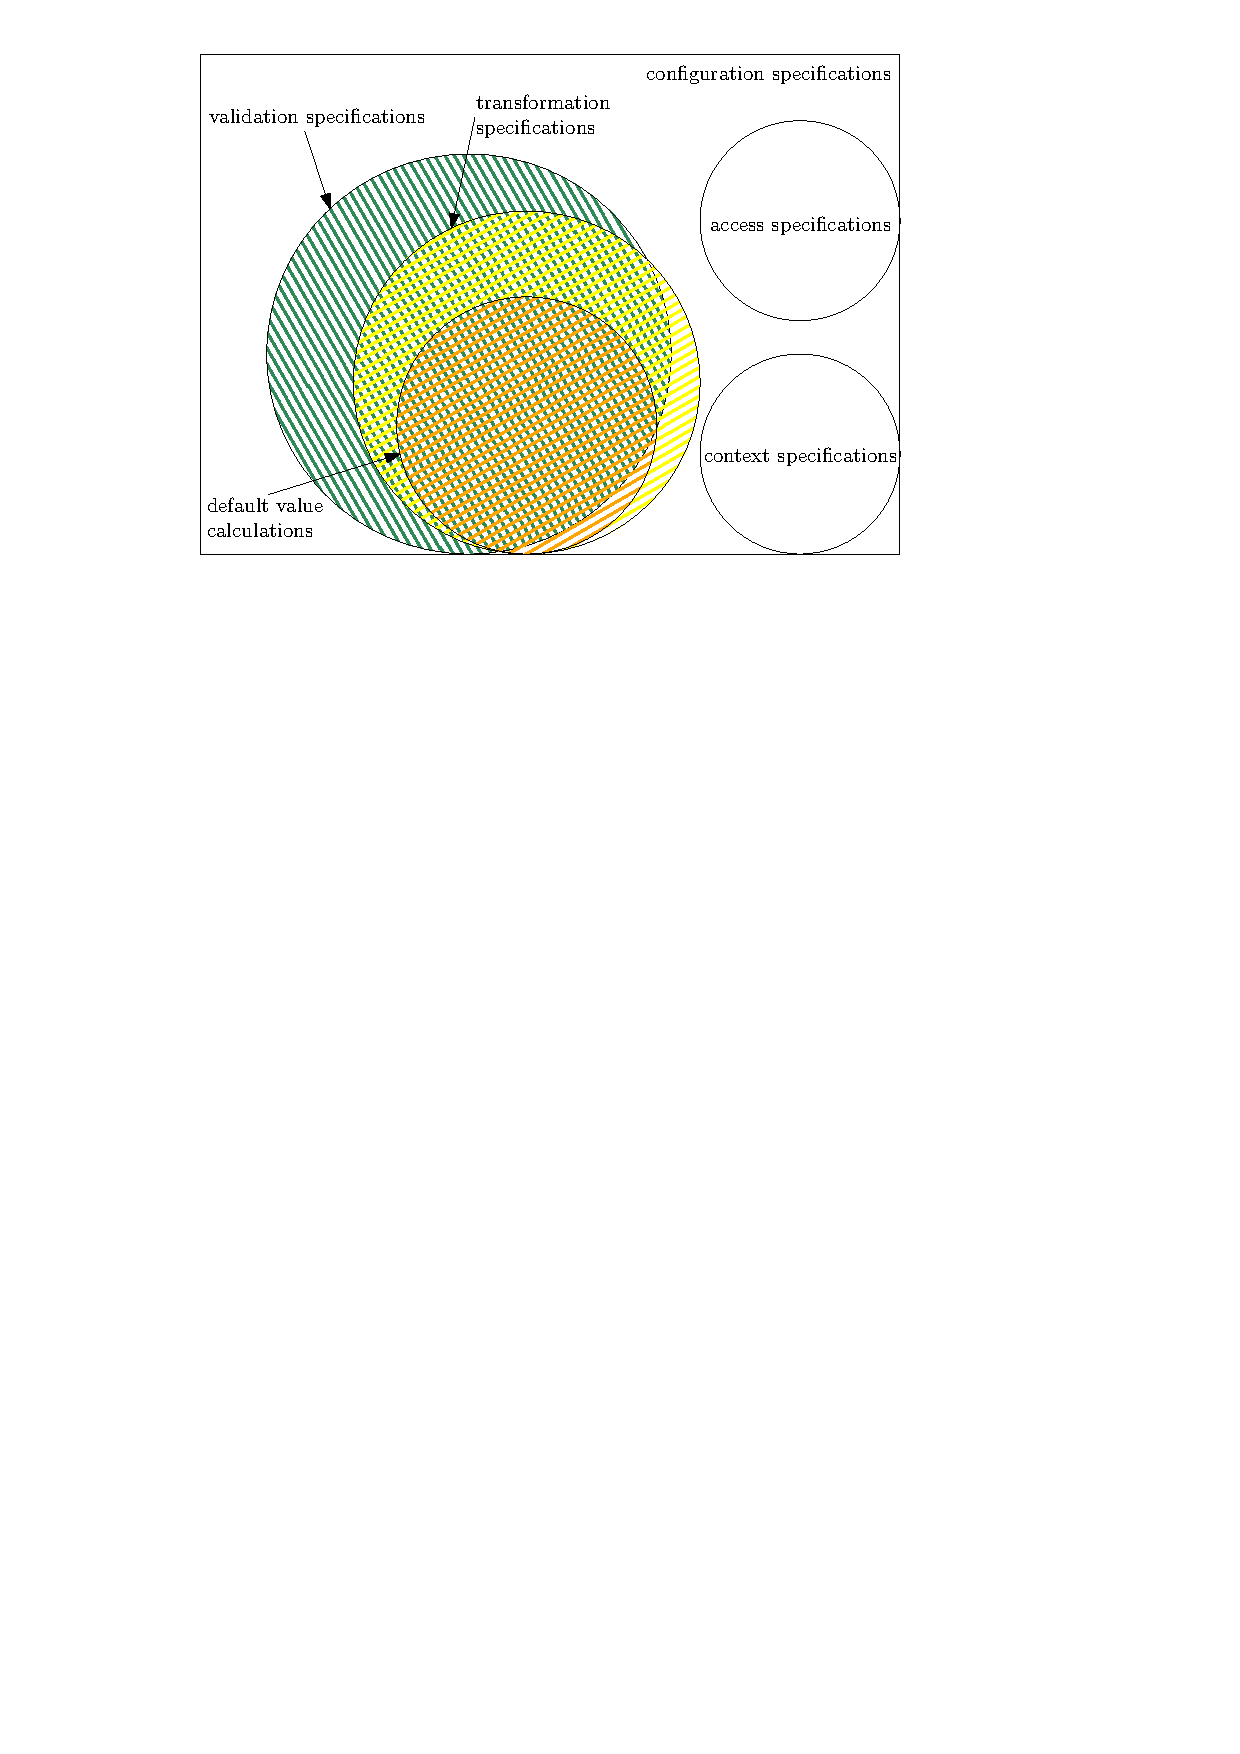
\includegraphics[scale=0.8]{specifications}
\end{frame}


\begin{frame}
	\frametitle{Requirements}

	\begin{itemize}
	\item formal/informal?
	\item complete?
	\pause
	\item should be extensible
	\item should be external to application
	\item open for introspection
	\item should talk to users
	\item should allow generation of artefacts
	\end{itemize}
\end{frame}


\begin{frame}[fragile]
	\frametitle{Grammar}
	\begin{grammar}
	<configuration specifications> ::= \{ <configuration specification> \}

	<configuration specification> ::= '[' <key> ']' <properties>

	<properties> ::= \{ <property> \}

	<property> ::= <property name> ':=' [ <property value> ]
	\end{grammar}

	\vspace{1cm}
	Example:
	\begin{code}[gobble=4]
	[slapd/threads/listener]
	default:=1
	type:=long
	\end{code}
\end{frame}


\section{Practise}

\begin{frame}
	\frametitle{Learning Outcomes}
	Students will be able to
	\begin{itemize}
	\item use configuration specification languages.
	\end{itemize}
\end{frame}

\begin{frame}
	\frametitle{Metalevels (Recapitulation)}
	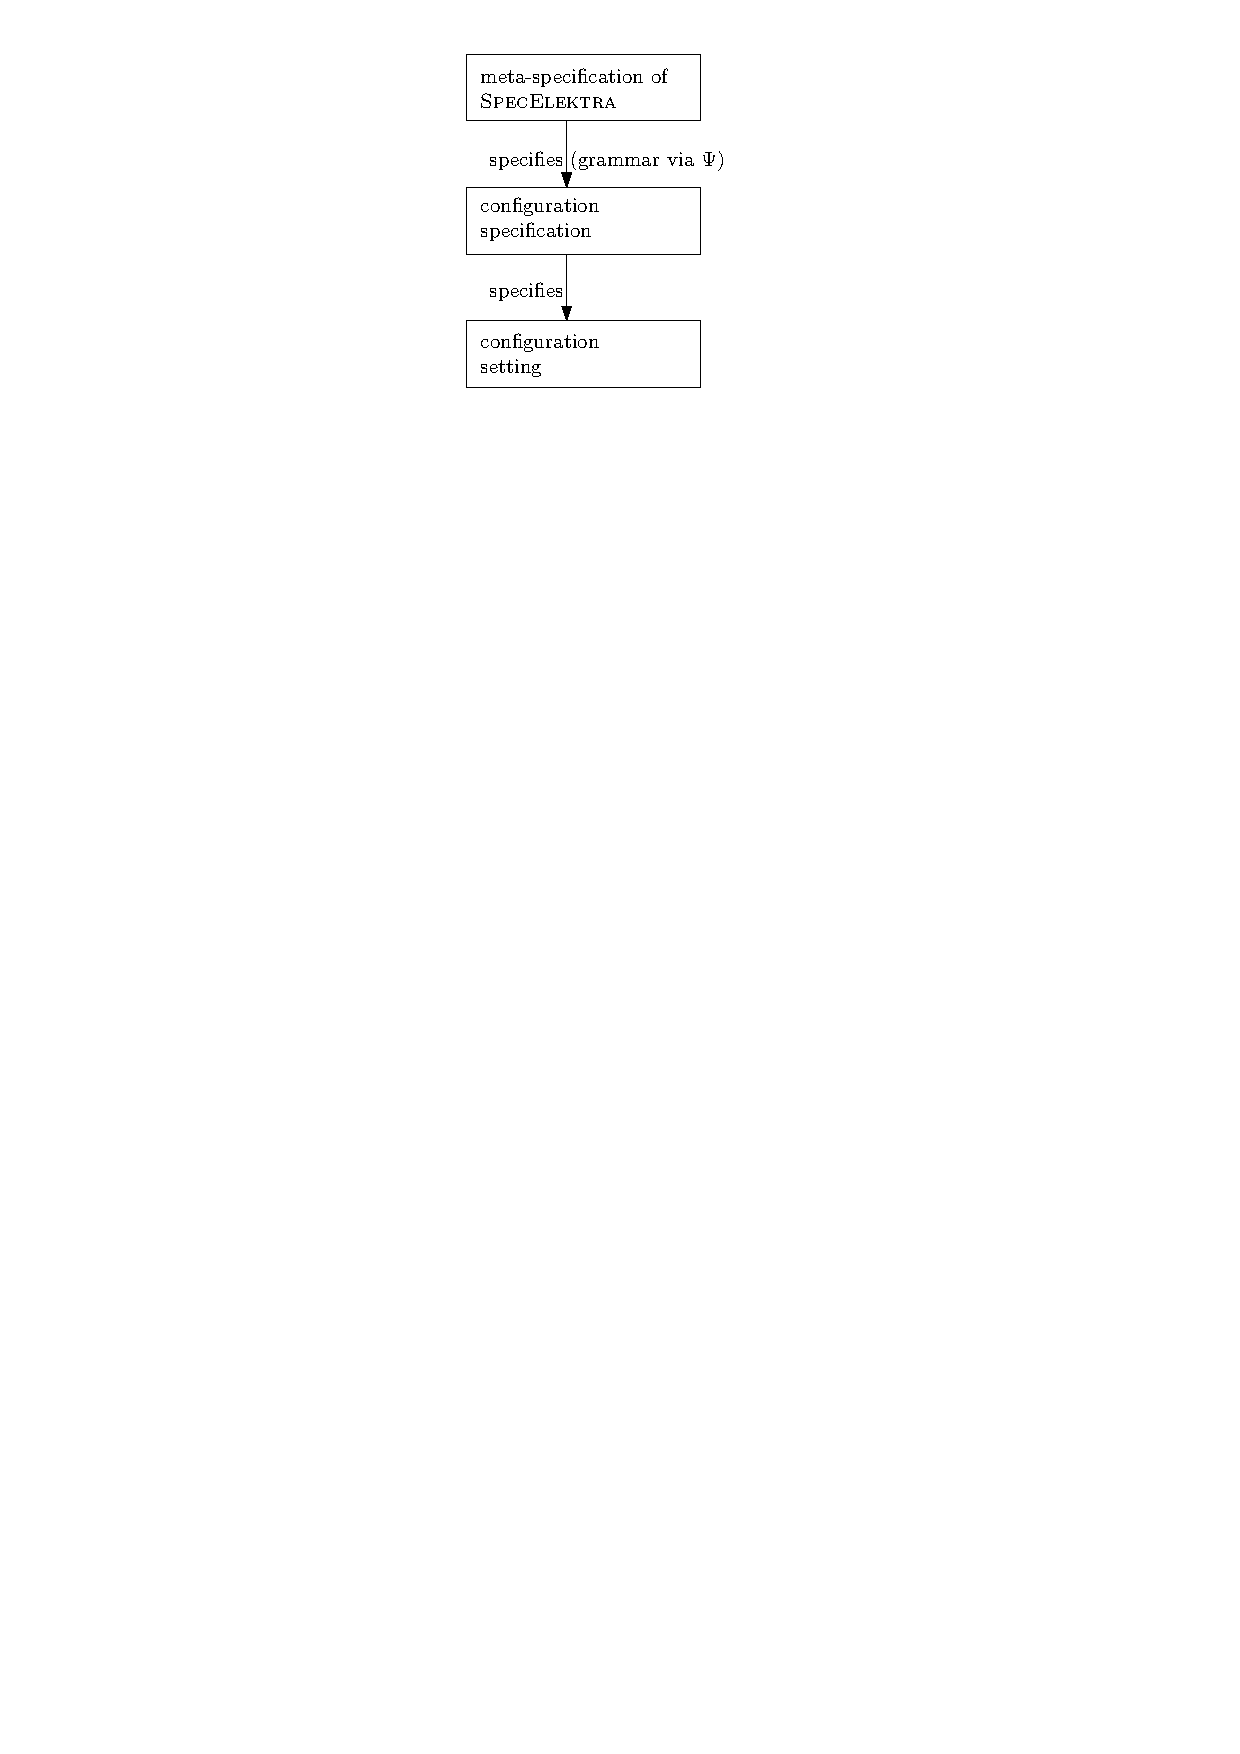
\includegraphics{metalevels}

	We will now walk through metalevels bottom-up.
\end{frame}

\begin{frame}[fragile]
	\frametitle{Configuration Settings (Recapitulation)}

	A configuration file may look like:

	\begin{code}[language=CfgElektra]
	a=5
	b=10
	c=15
	\end{code}

	We apply these configuration settings imperatively using:

	\begin{code}[language=bash]
	kdb set /a 5
	kdb set /b 10
	kdb set /c 15
	\end{code}

	And we list them with \lstinline[language=bash,morekeywords={ls},showspaces=no]^kdb ls /^.
\end{frame}

\begin{frame}[fragile]
	\frametitle{Specifications (Recapitulation)}
	For specifications such as:

	\begin{code}
	[slapd/threads/listener]
	  type:=short
	  default:=1
	\end{code}

	We apply the specifications imperatively using:

	\begin{code}[language=bash,morekeywords={meta,set,default}]
	kdb meta-set /slapd/threads/listener\
		type short
	kdb meta-set /slapd/threads/listener\
		default 1
	\end{code}

	(automatically uses ^spec:^ namespace)
\end{frame}

\begin{frame}[fragile]
	\frametitle{Meta-Specifications (Recapitulation)}
	For meta-specifications such as:

	\small
	\begin{code}[gobble=4]
	[type]
	type:=enum short unsigned_short long \
		float double char boolean any string ...
	description:=Defines the type of the value, \
		 as specified in CORBA
	\end{code}

	We apply the meta-specifications imperatively using:

	\begin{code}[language=bash,morekeywords={meta,set},gobble=4]
	kdb meta-set system:/info/elektra/metadata/type/#0 \
		type "enum short ..."
	kdb meta-set system:/info/elektra/metadata/type/#0 \
		description "Defines ..."
	\end{code}

	\large
	see ^doc/METADATA.ini^
\end{frame}

\begin{frame}
	\frametitle{SpecElektra}

	\begin{itemize}
	\item we use it to demonstrate configuration specification languages
	\item a modular \intro{specification language} for configuration settings
	\item we use properties to specify configuration settings and configuration access
	\item \elektra{Spec} specifies the behavior of \elektra{}
	\end{itemize}
\end{frame}


\begin{frame}[fragile]
	\frametitle{Mountpoint}

	The root of each configuration specification, e.g. in ni syntax:

	\begin{code}[morekeywords={mountpoint,infos,plugins},gobble=4]]
	[]
	mountpoint = vlc.ini
	infos/plugins = ni
	\end{code}
\end{frame}

\begin{frame}[fragile]
	\frametitle{Hierarchy}

	Always prefer hierarchy separator (^/^) as only separator:

	\begin{code}[gobble=4]
	[server/ip]
	\end{code}

	\vspace{1cm}

	Avoid other separators:

	\begin{code}[gobble=4]
	[server_ip]
	[server-ip]
	[server.ip]
	\end{code}

	Because they limit extensibility
	as they do not create sections in configuration files.
\end{frame}

\begin{frame}[fragile]
	\frametitle{Types}

	Presence alone indicates availability of a configuration setting:

	\begin{code}[gobble=4]
	[server/port]
	\end{code}

	Equivalent to ^type:=any^.

	\vspace{1cm}

	Properties give restrictions:

	\begin{code}[gobble=4]
	[server/port]
	type:=short
	\end{code}
\end{frame}

\begin{frame}[fragile]
	\frametitle{Require vs. Default}
	Prefer default values:
	\begin{code}[gobble=4]
	[server/ip]
	default:=127.0.0.1
	\end{code}

	Note that defaults must be sane and secure.

	\pause
	\vspace{1cm}

	Avoid require:

	\begin{code}[gobble=4]
	[server/ip]
	require:=
	\end{code}

	Because this forces the user to take action.
	\pause

	\begin{warn}
	\texttt{require and default} do not make sense together.
	\end{warn}
\end{frame}

\begin{frame}[fragile]
	\frametitle{IP Addresses}
	\begin{code}[morekeywords={ipaddr,example},gobble=4]
	[server/ip]
	check/ipaddr:=ipv4
	example:=0.0.0.0
	default:=127.0.0.1
	\end{code}

	Two plugins provide ^check/ipaddr^: ipaddr and network

	Will be automatically selected.
\end{frame}

\begin{frame}[fragile]
	\frametitle{Arrays}
	\begin{code}[gobble=4]
	[servers]
	array:=

	[servers/#/ip]
	check/ipaddr:=ipv4

	[servers/#/port]
	type:=short
	\end{code}
\end{frame}

\begin{frame}[fragile]
	\frametitle{Command-line Options}

	Environment and command-line options can be considered with:

	\begin{code}[morekeywords={long,env},gobble=4]]
	[recursive]
	  type:=boolean
	  opt:=r
	  opt/long:=recursive
	  env:=RECURSIVE
	  default:=0
	\end{code}
\end{frame}

\begin{frame}[fragile]
	\frametitle{Dates}
	\small
	\begin{code}[morekeywords={type,date,format,example},gobble=4]
	[mydate]
	example:=2021-03-01
	type:=string
	check/date:=ISO8601
	check/date/format:=calendardate complete extended
	\end{code}
\end{frame}

\begin{frame}[fragile]
	\frametitle{Design Considerations}
	Percentages
	\\ (e.g., configured image should be additionally cropped):
	\begin{code}[gobble=4]
	[image/width]
	type:=long

	[crop/width]
	type:=long
	check/range:=0-100
	\end{code}
\end{frame}

\begin{frame}
	\frametitle{Artefacts}
	\begin{itemize}
	\item plugins in configuration framework (e.g. validate settings)
	\item tooling (GUI, Web UI)
	\item generate examples/documentation
	\item auto-completion/syntax highlighting/IDE support
	\end{itemize}
\end{frame}




\section{Meeting}
\subsection{Recapitulation}

\begin{frame}
	\frametitle{Metalevels (Recapitulation)}
	\begin{alertblock}{Question}
	Describe the three Metalevels in Elektra.
	\end{alertblock}

	\pause
	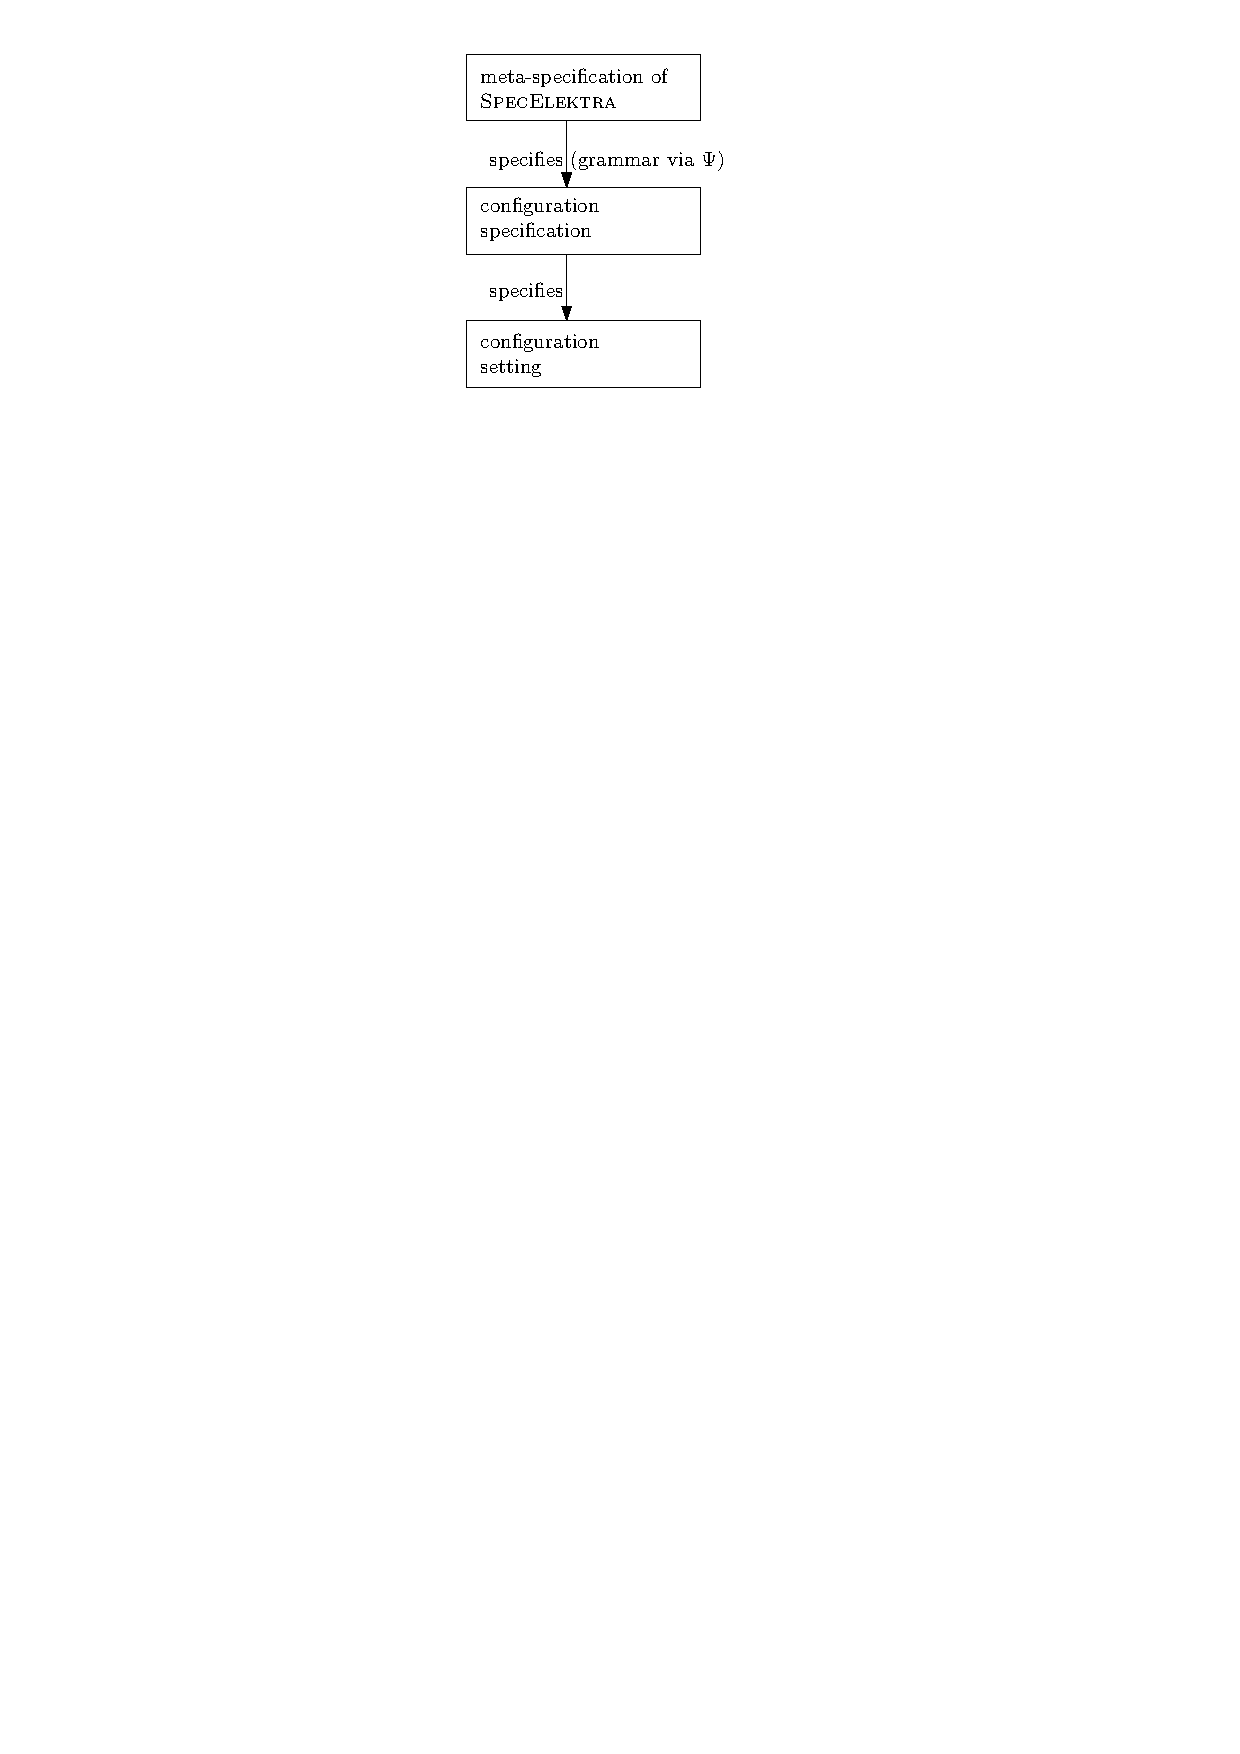
\includegraphics{metalevels}
\end{frame}

\begin{assignment}
	\begin{task}
	Is meta-data separated from or included in the data structure KeySet?
	\end{task}
\end{assignment}

\begin{assignment}
	\begin{task}
	Break.
	\end{task}
\end{assignment}

\begin{assignment}
	\begin{task}
	What do we mean with a configuration specification?
	\end{task}

	\begin{task}
	Which requirements do we have for a configuration specification?
	\end{task}

	\pause

	\begin{itemize}
	\item should be extensible
	\item should be external to application
	\item open for introspection (for tooling)
	\item should talk to users
	\item should allow generation of artefacts
	\end{itemize}
\end{assignment}

\begin{assignment}
	\begin{task}
	What can be part of a configuration specification?
	What can they be used for?
	\end{task}
\end{assignment}

\begin{assignment}
	\begin{task}
	Break.
	\end{task}
\end{assignment}

\begin{assignment}
	\begin{task}
	Now, how do we implement such a specification?
	Which artefacts can we generate?
	\end{task}
\end{assignment}

\subsection{Assignments}

\begin{frame}
	\frametitle{Develop with Elektra}

	\begin{task}
	Can you already compile software using Elektra?
	\end{task}
\end{frame}

\begin{frame}
	\frametitle{Teams}

	\begin{task}
	All Teams formed?
	\end{task}
\end{frame}

\begin{frame}
	\frametitle{Reformatting}

	\begin{task}
	Can you reformat the code?
	\end{task}
\end{frame}

\begin{frame}
	\frametitle{Running Tests}

	\begin{task}
	Can you run all the tests?
	\end{task}
\end{frame}

\subsection{L03: Configuration Integration}

\begin{frame}
	\frametitle{Preview Next Week}

	\begin{itemize}
	\item Configuration Libraries
	\item Lightweight to Strong Integration
	\item Sharing Configuration
	\end{itemize}
\end{frame}




%%%%%%%%%%%%%%%%%%%%%%%%%%%%%%%%%%%%%%%%%% 
\nocite{raab2017introducing}

\appendix

\begin{frame}[allowframebreaks]
	\bibliographystyle{plainnat}
	\bibliography{../shared/elektra.bib}
\end{frame}

\end{document}


